\documentclass[journal,12pt,twocolumn]{IEEEtran}

\usepackage{setspace}
\usepackage{gensymb}

\singlespacing
\usepackage{pstricks}
\usepackage[cmex10]{amsmath}
%\usepackage{amsthm}
%\interdisplaylinepenalty=2500
%\savesymbol{iint}
%\usepackage{txfonts}
%\restoresymbol{TXF}{iint}
%\usepackage{wasysym}
\usepackage{amsthm}
%\usepackage{iithtlc}
\usepackage{mathrsfs}
\usepackage{txfonts}
\usepackage{stfloats}
\usepackage{bm}
\usepackage{cite}
\usepackage{cases}
\usepackage{subfig}
%\usepackage{xtab}
\usepackage{longtable}
\usepackage{multirow}
%\usepackage{algorithm}
%\usepackage{algpseudocode}
\usepackage{enumitem}
\usepackage{mathtools}
\usepackage{caption}
\usepackage{steinmetz}
\usepackage{tikz}
%\usepackage{circuitikz}
\usepackage{verbatim}
\usepackage{tfrupee}
\usepackage[breaklinks=true]{hyperref}
%\usepackage{stmaryrd}
\usepackage{tkz-euclide} % loads  TikZ and tkz-base
%\usetkzobj{all}
\usetikzlibrary{calc,math}
\usepackage{listings}
\usepackage{color}                                            %%
\usepackage{array}                                            %%
\usepackage{longtable}                                        %%
\usepackage{calc}                                             %%
\usepackage{multirow}                                         %%
\usepackage{hhline}                                           %%
\usepackage{ifthen}                                           %%
%optionally (for landscape tables embedded in another document): %%
\usepackage{lscape}     
%\usepackage{multicol}
\usepackage{chngcntr}
%\usepackage{enumerate}
%\usepackage{wasysym}
%\newcounter{MYtempeqncnt}
\DeclareMathOperator*{\Res}{Res}
%\renewcommand{\baselinestretch}{2}
\renewcommand\thesection{\arabic{section}}
\renewcommand\thesubsection{\thesection.\arabic{subsection}}
\renewcommand\thesubsubsection{\thesubsection.\arabic{subsubsection}}

\renewcommand\thesectiondis{\arabic{section}}
\renewcommand\thesubsectiondis{\thesectiondis.\arabic{subsection}}
\renewcommand\thesubsubsectiondis{\thesubsectiondis.\arabic{subsubsection}}

% correct bad hyphenation here
\hyphenation{op-tical net-works semi-conduc-tor}
\def\inputGnumericTable{}                                 %%

\lstset{
	%language=C,
	frame=single, 
	breaklines=true,
	columns=fullflexible
}
\usepackage{amssymb}
\usepackage{stackengine}
\usepackage{scalerel}
\usepackage{graphicx}
\newlength\lthk
\setlength\lthk{.1ex}
\def\bline{\rule{2ex}{\lthk}}
\def\slash{\rotatebox{60}{\bline}}
\def\parallelogram{\stackMath\scalerel*{%
		\def\stackalignment{l}{\stackunder[-.5\lthk]{%
				\def\stackalignment{r}\stackon[-.5\lthk]{\slash\rule{.866ex}{0ex}\slash}{\bline}}%
			{\bline}}}{\square}%
}

\begin{document}
	%
	
	
	\newtheorem{theorem}{Theorem}[section]
	\newtheorem{problem}{Problem}
	\newtheorem{proposition}{Proposition}[section]
	\newtheorem{lemma}{Lemma}[section]
	\newtheorem{corollary}[theorem]{Corollary}
	\newtheorem{example}{Example}[section]
	\newtheorem{definition}[problem]{Definition}
	
	\newcommand{\BEQA}{\begin{eqnarray}}
		\newcommand{\EEQA}{\end{eqnarray}}
	\newcommand{\define}{\stackrel{\triangle}{=}}
	\bibliographystyle{IEEEtran}
	%\bibliographystyle{ieeetr}
	\providecommand{\mbf}{\mathbf}
	\providecommand{\pr}[1]{\ensuremath{\Pr\left(#1\right)}}
	\providecommand{\qfunc}[1]{\ensuremath{Q\left(#1\right)}}
	\providecommand{\sbrak}[1]{\ensuremath{{}\left[#1\right]}}
	\providecommand{\lsbrak}[1]{\ensuremath{{}\left[#1\right.}}
	\providecommand{\rsbrak}[1]{\ensuremath{{}\left.#1\right]}}
	\providecommand{\brak}[1]{\ensuremath{\left(#1\right)}}
	\providecommand{\lbrak}[1]{\ensuremath{\left(#1\right.}}
	\providecommand{\rbrak}[1]{\ensuremath{\left.#1\right)}}
	\providecommand{\cbrak}[1]{\ensuremath{\left\{#1\right\}}}
	\providecommand{\lcbrak}[1]{\ensuremath{\left\{#1\right.}}
	\providecommand{\rcbrak}[1]{\ensuremath{\left.#1\right\}}}
	\theoremstyle{remark}
	\newtheorem{rem}{Remark}
	\newcommand{\sgn}{\mathop{\mathrm{sgn}}}
	\providecommand{\abs}[1]{\left\vert#1\right\vert}
	\providecommand{\res}[1]{\Res\displaylimits_{#1}} 
	\providecommand{\norm}[1]{\left\lVert#1\right\rVert}
	%\providecommand{\norm}[1]{\lVert#1\rVert}
	\providecommand{\mtx}[1]{\mathbf{#1}}
	\providecommand{\mean}[1]{E\left[ #1 \right]}
	\providecommand{\fourier}{\overset{\mathcal{F}}{ \rightleftharpoons}}
	%\providecommand{\hilbert}{\overset{\mathcal{H}}{ \rightleftharpoons}}
	\providecommand{\system}{\overset{\mathcal{H}}{ \longleftrightarrow}}
	%\newcommand{\solution}[2]{\textbf{Solution:}{#1}}
	\newcommand{\solution}{\noindent \textbf{Solution: }}
	\newcommand{\cosec}{\,\text{cosec}\,}
	\providecommand{\dec}[2]{\ensuremath{\overset{#1}{\underset{#2}{\gtrless}}}}
	\newcommand{\myvec}[1]{\ensuremath{\begin{pmatrix}#1\end{pmatrix}}}
	\newcommand{\mydet}[1]{\ensuremath{\begin{vmatrix}#1\end{vmatrix}}}
	%\numberwithin{equation}{section}
	\numberwithin{equation}{subsection}
	%\numberwithin{problem}{section}
	%\numberwithin{definition}{section}
	\makeatletter
	\@addtoreset{figure}{problem}
	\makeatother
	\let\StandardTheFigure\thefigure
	\let\vec\mathbf
	%\renewcommand{\thefigure}{\theproblem.\arabic{figure}}
	\renewcommand{\thefigure}{\theproblem}
	%\setlist[enumerate,1]{before=\renewcommand\theequation{\theenumi.\arabic{equation}}
	%\counterwithin{equation}{enumi}
	%\renewcommand{\theequation}{\arabic{subsection}.\arabic{equation}}
	\def\putbox#1#2#3{\makebox[0in][l]{\makebox[#1][l]{}\raisebox{\baselineskip}[0in][0in]{\raisebox{#2}[0in][0in]{#3}}}}
	\def\rightbox#1{\makebox[0in][r]{#1}}
	\def\centbox#1{\makebox[0in]{#1}}
	\def\topbox#1{\raisebox{-\baselineskip}[0in][0in]{#1}}
	\def\midbox#1{\raisebox{-0.5\baselineskip}[0in][0in]{#1}}
	\vspace{3cm}
	\title{Assignment-6}
	\author{Pooja H \\ AI20MTECH14003}
	\maketitle
	\newpage
	\bigskip
	\renewcommand{\thefigure}{\theenumi}
	\renewcommand{\thetable}{\theenumi}
\begin{abstract}
	In this document, we find the value of k such that the equation represents a pair of straight lines.
\end{abstract}
%Download all python codes from 
%\begin{lstlisting}
%	https://github.com/poojah15/EE5609_AI20MTECH14003/tree/master/Assignment_6
%\end{lstlisting}
Download all latex-tikz codes from 
\begin{lstlisting}
	https://github.com/poojah15/EE5609_AI20MTECH14003/tree/master/Assignment_6
\end{lstlisting}
\section{Problem Statement}
Find the value of k such that $6x^2 + 11xy - 10y^2 + x + 31y + k =0$ represent pairs of straight lines.
\section{Theory}
The general equation of second degree is given by 
\begin{align} 
	ax^2 + 2bxy + cy^2 + 2dx + 2ey + f = 0 
\end{align}
and can be expressed as 
\begin{align}
	\vec{x}^T\vec{Vx} + 2\vec{u}^T\vec{x} + f = 0 \label{eq:eq1}
\end{align}
where 
\begin{align}
	\vec{V} = \vec{V}^T = \myvec{a & b\\b & c} \label{eq:eq2} \\
	\vec{u}^T = \myvec{d & e} \label{eq:eq3}
\end{align}
Let the pair of straight lines be given by 
\begin{align}
	\vec{n}_1^T\vec{x} = c_1\\
	\vec{n}_2^T\vec{x} = c_2
\end{align}
Equating their product with \eqref{eq:eq1}, we get
\begin{align}
	(\vec{n}_1^T\vec{x} - c_1)(\vec{n}_2^T\vec{x} - c_2) \nonumber \\
	\implies \vec{x}^T\vec{Vx} + 2\vec{u}^T\vec{x} + f = 0 \label{eq:eq4}
\end{align}
\eqref{eq:eq4} represents a pair of straight lines if
\begin{align} \label{eq:det1}
	\mydet{\vec{V} & \vec{u} \\ \vec{u}^T & f} = 0
\end{align}
\section{Solution}
Given, 
\begin{align}
	6x^2 + 11xy - 10y^2 + x + 31y + k =0 \label{eq:eq5}
\end{align}
Equating  \eqref{eq:eq5} to \eqref{eq:eq1}, we get
\begin{align}
	\vec{V} = \myvec{6 & \frac{11}{2} \\ \frac{11}{2} & -10}\\
	\vec{u}^T = \myvec{\frac{1}{2} & \frac{31}{2}}
\end{align}
Substituting $\vec{V}$ and $\vec{u}^T$ in \eqref{eq:det1}, we obtain
\begin{align}
\mydet{6 & \frac{11}{2} & \frac{1}{2} \\ \frac{11}{2} & -10 & \frac{31}{2} \\ \frac{1}{2} & \frac{31}{2} & k} = 0 \\
\implies 6\brak{-10k - \brak{\frac{31}{2}}^2}-\frac{11}{2}\brak{\frac{11}{2}k - \frac{31}{4}} \nonumber\\+ \frac{1}{2}\brak{\frac{11}{2}\times\frac{31}{2} +5} = 0\\
\implies \frac{-361}{4}k - \frac{5415}{4} = 0\\
\implies \boxed{k = -15} \label{eq:res}
\end{align}
Substituting \eqref{eq:res} in \eqref{eq:eq5}, we get
\begin{align}
	6x^2 + 11xy - 10y^2 + x + 31y - 15 =0 \label{eq:reseq}
\end{align}
Hence the solution.
\section{Graphical Illustration}
Firstly, obtain linear equation of the form ($ax + by + c$) of \eqref{eq:reseq} by considering
\begin{align}
	6x^2 + 11xy - 10y^2 \\
	\implies 6x^2 - 4xy + 15xy - 10y^2\\
	\implies 2x(3x - 2y) + 5y(3x - 2y)\\
	\implies (3x - 2y)(2x + 5y) \label{eq:factor}
\end{align}
Equation \eqref{eq:factor} can be written as,
\begin{align}
	(3x - 2y + m)(2x + 5y + n) &= 0 \label{eq:mn} \\
	\implies 6x^2 + 11xy - 10y^2 + (3n + 2m)x \nonumber \\+ (-2n + 5m)y &= 0 \label{eq: eqmn}
\end{align}
Equating \eqref{eq:reseq} and \eqref{eq: eqmn},
\begin{align}
	3n + 2m &= 1\\
	-2n + 5m &= 31
\end{align}
Solving for m and n we obtain,
\begin{align}
	m &= 5 \label{eq:mval} \\
	n &= -3 \label{eq:nval}
\end{align}
Substituting \eqref{eq:mval} and \eqref{eq:nval} in \eqref{eq:mn}, we obtain
\begin{align}
	(3x - 2y + 5)(2x + 5y - 3) = 0 \label{eq:finalres}
\end{align}
Hence \eqref{eq:finalres} represent equation of two straight lines.
Graphically,
\renewcommand{\thefigure}{\arabic{figure}}
\begin{figure}[!ht] \label{fig:straight_lines}
	\centering
	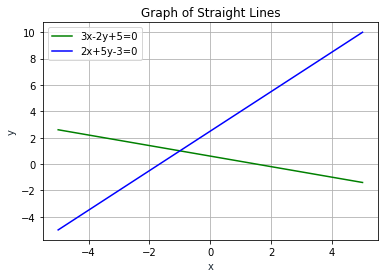
\includegraphics[width=\columnwidth]{a6_graph.png}
	\caption{Plot of two straight lines.}
\end{figure}
\end{document}